\section{Introduction}
The Kicad 3D Models project aims to produce high-quality parametric models for use
with KiCAD.  Initially these will be VRML2.0 models for use in the KiCAD 3D Viewer
but as the Free-CAD project matures, Free-CAD solid models will also be added with
the intention of providing a means of generating a solid model of the board to aid
users with their mechanical integration requirements.

This document describes the installation and use of the Python modules for generating
VRML models from existing parametric models as well as how to use the existing
parameterized features from the toolbox to create new parametric models within Python.

For an introduction to using VRML2.0 with KiCAD, see the document \emph{kicad\_3d\_vrml.pdf}
``Tutorial: VRML2.0 and KiCAD'' and references therein.

This document assumes the user is familiar with the VRML2.0 specification and the
current limitations of the KiCAD 3D viewer which restrict the VRML features used
in the 3D models. The user is also assumed to have a basic familiarity with
the GNU compiler and the Python interpreter.

This tutorial is aimed at users with a GNU/Linux system since the source code has
been developed on such a system; users with experience on other systems are
encouraged to make appropriate adjustments to the source code and build tools and
to report results to the author via the project website (http://kicad3dmodels.sourceforge.net).

To view the VRML models, use a viewer such as \verb#whitedune# on Linux or \verb#Cortona3D#
on MSWindows.

\section{Installation}
The current requirements for installation of the Kicad 3D parametric models are:
\begin{itemize}
\item git version 1.7 or later (earlier versions may work)\\
\item Kicad3DModels source code\\
\item GNU C++ compiler\\
\item CMake version 2.8 or later (earlier versions may work)\\
\item Python version 2.6 or later\\
\item Boost::Python version 1.49 or later (earlier versions may work)\\
\end{itemize}

To retrieve the source code via git, change to your preferred working directory
then invoke git to create the project's subdirectory:

\verb#git clone git://git.code.sf.net/p/kicad3dmodels/code kicad3d#

Change to the top level project directory:

\verb#cd kicad3d#

The project uses the CMake build tool and each subdirectory contains a
\verb#CMakeLists.txt# file with instructions for CMake. Since the 
instructions to build the Python bindings depends on the specific setup
of your system, you will need to edit the file \verb#src/py/CMakeLists.txt#
and check the following:

\verb#SET(ENV{BOOST_ROOT} "/usr/lib")# Set the path to your BOOST installation

\verb#SET(PYTHON_INCLUDE "/usr/include/python2.7")# Set the path to the header
files for the version of Python you wish to use.

\verb#SET(PYTHON_VERSION python2.7)# Set to the version of Python you wish to use.

\verb#find_package(Boost 1.49 EXACT REQUIRED COMPONENTS python)# Set the BOOST version
to the version installed on your system.

Once those changes are made we should be ready to configure and build the tools.
To keep the source tree free of temporary build files, we will create a build
directory in the top level project directory (\verb#kicad3d#) then build and install
the files:

\begin{verbatim}
mkdir build
cd build
cmake ..
sudo make install
sudo ldconfig
\end{verbatim}

The various tools and libraries will be built; executable files will be installed within
the \verb#/usr/local/bin# directory in the project tree and the shared libraries,
including Python modules, will be installed within the \verb#/usr/local/lib# directory.
Material appearance specifications will be installed in \verb#/usr/local/share/mcad/colors#.

To check that everything is fine, set the
\verb#PYTHONPATH# environment variable to include the \verb#/usr/local/lib# directory.
This can be done via the command ``\verb#export PYTHONPATH=/usr/local/lib#''.
We should now be able to load the modules from within Python:

\begin{verbatim}
python
Python 2.7.3rc2 (default, Apr 22 2012, 22:35:38) 
[GCC 4.6.3] on linux2
Type "help", "copyright", "credits" or "license" for more information.
>>> import kc3d
>>> import kc3dconn
\end{verbatim}

Some executables such as \verb#makeDip#,  \verb#make19950#,  and
\verb#makePCC-SMP# assume that the material appearance definitions
are in the directory \verb#/usr/local/share/mcad/colors# and will
fail if the definitions are not present.

\section{Quick Example}
\label{sec:quick-example}
In this brief example we will invoke a single parametric model to
build a variety of 6x2 DIL headers as a demonstration of the
flexibility of parametric models.

For consistency in the appearance of materials in the models, material
appearances are defined in files within the directory \verb#mcad/colors#.
For the convenience of this exercise and all future exercises in this
tutorial, we will create models from the directory \verb#mcad/test#.
To set up, execute the following commands:

\begin{verbatim}
mkdir mcad
cd mcad
ln -s /usr/local/share/mcad/colors .
mkdir test
cd test
\end{verbatim}

create the test directory and change to it. Ensure that the PYTHONPATH
had been set as discussed in the section on installing the software.
All future examples in this tutorial will assume that the working
directory is \verb#mcad/test#.
Run Python and execute the following Python commands (ignore lines
beginning with `\#' - these are merely code comments):

\begin{verbatim}
# load the tools
import kc3d
import kc3dconn
from kc3d import *
from kc3dconn import *

# instantiate necessary objects
out = ofstream()
hdr = Genhdr()
tx = Transform()
# set the scale to 1/2.54 so that the VRML units correspond to
# the 0.1 inch used by KiCAD.
tx.setScale(0.3937)

# create a male 6x2 header with square pins 8mm high, 2.54mm pitch, and beveled case
SetupVRML("testhdr_MS_6x2_8mm.wrl", out)
hdr.setColors("../colors/black.mat", "../colors/gold.mat", "../colors/gold.mat",
    "../colors/tin.mat")
hdr.setCase(6, 2, 2.54, 2.54, 2.72, 0.72, True, 0.3)
hdr.setPins(True, True, True, -1, -1, 2, 10, 0.64, 0.64, 0, 0, 0, 0, 0.3, 0.8, 4, 0)
hdr.build(tx, "HDR_MALE_SP_6x2_8MM", out, 0)
out.close()

# create a female 6x2 header with square pins, 8mm high beveled case, 2.54mm pitch
kc3d.SetupVRML("testhdr_FS_6x2_8mm.wrl", out)
hdr.setColors("../colors/black.mat", "../colors/tin.mat", "../colors/gold.mat",
    "../colors/black.mat")
hdr.setCase(6, 2, 2.54, 2.54, 8, 0.72, True, 0.3)
hdr.setPins(True, True, False, -1, -1, 2, 10, 0.64, 0.64, 1.6,
    1.09, 0, 0, 0.3, 0.8, 24, 0.5)
hdr.build(tx, "HDR_FEMALE_SP_6x2_8MM", out, 0)
out.close()

# create a female 6x2 header with round pins, 8mm high beveled case, 2.54mm pitch
kc3d.SetupVRML("testhdr_FR_6x2_8mm.wrl", out)
hdr.setCase(6, 2, 2.54, 2.54, 8, 0.72, True, 0.3)
hdr.setPins(False, False, False, -1, -1, 2, 10, 0.64, 0.64, 1.6,
    0.84, 1.32, 1.2, 0.3, 0.8, 24, 0.5)
hdr.build(tx, "HDR_FEMALE_RP_6x2_8MM", out, 0)
out.close()
\end{verbatim}

Exit the python interpreter and inspect the model files with a VRML viewer.
This is only a very brief introduction to a parametric model. For this
particular model (\verb#Genhdr#), many parameters can be changed to produce
a different model - for example, the number of rows or columns can be changed
and the case can be plain with no bevel. The model only produces vertical
headers with straight pins but the model itself relies on other components
which describe the shape of a pin and the shape of the case; these more
basic components can be used to create models for generating 90-degree
headers, SMD headers, and so on.

\begin{figure}
\label{fig:k3dintro-headers}
\centering
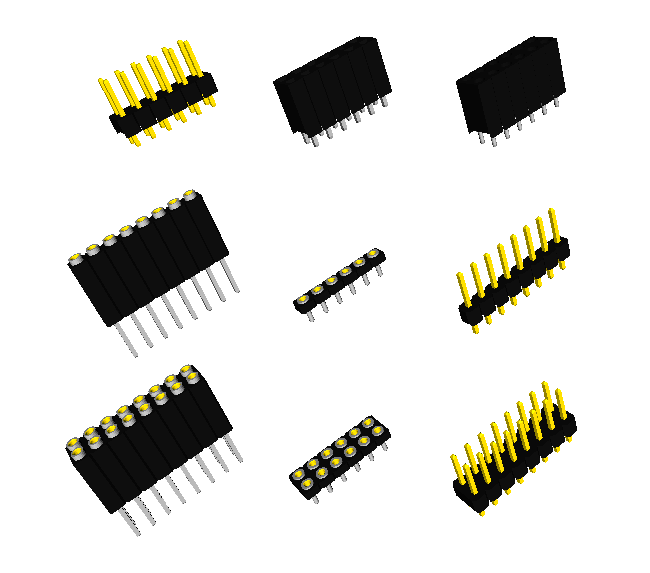
\includegraphics[width = 0.6\textwidth]{img/k3dintro-headers.png}
\caption{A sample of headers generated by the Genhdr object.}
\end{figure}
